%========================================================
% Reusable academic paper template
% Preserves the overall look and feel of the uploaded draft
% while removing the original paper-specific content.
%
% Quick start:
% 1. Replace the metadata block below.
% 2. Set \blindtrue for anonymized (blind-review) output, or \blindfalse to show authors.
% 3. Replace the sample text, tables, and figures.
% 4. Replace the .bib file with your own references.
% 5. Compile with: pdflatex -> bibtex -> pdflatex -> pdflatex
%========================================================

\documentclass[hidelinks,12pt]{article}

\usepackage{graphicx}
\usepackage{setspace}
\usepackage[svgnames]{xcolor}
\usepackage[colorlinks=true,citecolor=DarkBlue,linkcolor=Maroon]{hyperref}
\usepackage{fancyhdr}
\usepackage{natbib}
\usepackage[format=hang,font=large,labelfont=bf]{caption}
\usepackage{tabularx}
\usepackage{booktabs,multicol,multirow}
\usepackage[margin=2cm]{geometry}
\usepackage{array}
\usepackage{amsmath}
\usepackage{enumitem}
\usepackage[toc,page]{appendix}

\captionsetup[table]{labelsep=period}
\captionsetup[figure]{labelsep=period}

\newcolumntype{Y}{>{\raggedleft\arraybackslash}X}
\newcolumntype{L}[1]{>{\raggedright\let\newline\\\arraybackslash\hspace{0pt}}m{#1}}

\def\sym#1{\ifmmode^{#1}\else\(^{#1}\)\fi}

% Capitalized autoref names for clickable cross-references
\renewcommand{\figureautorefname}{Figure}
\renewcommand{\tableautorefname}{Table}
\renewcommand{\sectionautorefname}{Section}
\renewcommand{\subsectionautorefname}{Section}
\newcommand{\propositionautorefname}{Proposition}
\newcommand{\hypothesisautorefname}{Hypothesis}
\newcommand{\appendixautorefname}{Appendix}

\newcommand{\runningtitle}{Academic Paper Template}
\newcommand{\papertitle}{Reusable Academic Paper Template: Example Layout for Empirical Research}
\newcommand{\paperauthorone}{First Author}
\newcommand{\paperauthortwo}{Second Author}
\newcommand{\paperaffilone}{Department of Finance, University A}
\newcommand{\paperaffiltwo}{Department of Economics, University B}
\newcommand{\paperemailone}{first.author@university.edu}
\newcommand{\paperemailtwo}{second.author@university.edu}

\newif\ifblind
\blindfalse % change to \blindtrue for anonymized (blind-review) output

\newcommand{\floatnotes}[1]{%
\begin{quotation}
\noindent \scriptsize #1
\end{quotation}
}

\renewcommand{\baselinestretch}{1.9}
\setlength{\textheight}{8.6in}
\setlength{\textwidth}{6.3in}
\setlength{\oddsidemargin}{0.1in}
\setlength{\topmargin}{-0.30in}
\setlength{\footnotesep}{10.0pt}
\setlength{\headheight}{14.5pt}

\pagestyle{fancyplain}
\fancyhf{}
\lhead{\textbf{\runningtitle}}
\rhead{\thepage}
\renewcommand{\headrulewidth}{0.4pt}
\renewcommand{\footrulewidth}{0pt}

\title{\bf \papertitle\\
\vspace*{-20pt}}
\author{}
\date{}

\begin{document}

\maketitle
\thispagestyle{empty}

\ifblind\else
\vspace{-1.5em}
\begin{center}
\paperauthorone\\
\textit{\paperaffilone}\\
\href{mailto:\paperemailone}{\paperemailone}
\vspace{0.7em}

\paperauthortwo\\
\textit{\paperaffiltwo}\\
\href{mailto:\paperemailtwo}{\paperemailtwo}
\end{center}
\vspace{1.0em}
\fi

\begin{abstract}
\vspace{0pt}
\setstretch{1.15}
This document is a reusable template that keeps the general appearance of the uploaded draft while removing the original paper-specific material. It includes a sample title page, abstract, section structure, equations, hypotheses, references, tables, figures, and an appendix. The example prose is written around a stylized empirical finance question on disclosure quality and financing costs, but every number, coefficient, table entry, and graphic is illustrative only. Replace the metadata, narrative, variable names, sample description, notes, and bibliography with your own project-specific content before submission.
\end{abstract}

\setstretch{1.9}

\vspace{32pt}
{\noindent JEL Classification: } G10, G30, C23\\
Keywords: academic template; empirical finance; disclosure; financing costs

\newpage
\setcounter{page}{1}

%--------------------------------------------------------
\section{Introduction}
\label{sec:intro}

A strong introduction usually does four things in quick succession: it states the research question, explains why the question matters, positions the paper relative to the literature, and previews the empirical design and the main findings. This template illustrates that structure with placeholder content built around a stylized relation between disclosure quality and financing costs. Replace the topic, motivation, and contribution statements with the central question in your own paper.

For illustration, suppose the paper studies whether better disclosure lowers financing frictions by improving investor understanding and reducing information asymmetry. That framing fits naturally with prior work on disclosure and the cost of capital, including \citet{botosan1997disclosure}, \citet{healy2001information}, and \citet{lambert2007accounting}. A finance paper might then connect the question to broader asset-pricing or corporate-finance themes such as risk premia, monitoring, or capital structure, perhaps citing benchmark references like \citet{fama1993common} or \citet{jensen1976theory}.

A second paragraph in the introduction typically explains the research design at a high level. Here, the placeholder design uses panel regressions with firm and year fixed effects, standard controls, and clustered standard errors following \citet{petersen2009estimating}. It also flags endogeneity concerns and previews the kinds of robustness checks discussed by \citet{angrist2009mostly}.\footnote{Use footnotes sparingly. They work best for brief institutional details, measurement clarifications, or secondary discussion that would otherwise interrupt the main argument.}

A third paragraph often summarizes the paper's contributions. In a completed draft, this is where you would explain what is new relative to prior work, why the data or identification strategy is informative, and how the magnitudes matter economically. The sample tables/figures at the end of the document show common formatting choices for descriptive statistics, baseline regressions, heterogeneity tests, and visual summaries. For example, \autoref{tab:summary} presents summary statistics, \autoref{tab:baseline} presents a baseline regression layout, and \autoref{fig:binned_scatter} shows a standard binned-scatter figure.

The remainder of the paper proceeds as follows. \autoref{sec:literature} illustrates how to position the study in the literature and develop hypotheses. \autoref{sec:data} describes the sample and variable construction. \autoref{sec:design} presents an example empirical specification. \autoref{sec:results} and \autoref{sec:additional} show a typical flow for main results, heterogeneity, and robustness. The appendix provides an example supplementary section and a variable-definition table.

%--------------------------------------------------------
\section{Related Literature and Hypothesis Development}
\label{sec:literature}

\subsection{Delegated Portfolio Management and Fund Performance}

The question of whether mutual fund managers possess investment skill has generated a large and contested literature. \citet{grinblatt1992persistence} provide early evidence that fund performance persists over short horizons, but \citet{carhart1997persistence} demonstrates that most apparent persistence is attributable to common factors in stock returns and investment expenses rather than managerial ability. The only robust persistence pattern is that the worst-performing funds continue to underperform, consistent with high costs and poor governance rather than bad luck. \citet{brown1995performance} reach a similar conclusion using survivorship-bias-free samples, finding that persistence concentrates in underperformance. More recently, \citet{kaniel2023machine} apply machine learning methods to isolate fund manager skill and find that a meaningful minority of managers do generate persistent alpha, though the average fund does not.

A separate line of work examines why funds that lack skill survive. \citet{song2020mismatch} shows that many investors confuse systematic factor exposures with managerial skill, causing oversized funds to accumulate assets well beyond their capacity to generate alpha. The result is a mismatch between scale and skill that explains much of the aggregate underperformance of active management. \citet{bogle2005mutual} documents the broader industry trend: total mutual fund assets have grown 3,600-fold since 1945, but fees and expenses have grown 6,600-fold, suggesting that industry growth has benefited fund managers more than fund shareholders.

These findings raise a governance question that the performance literature largely leaves unanswered: if most active funds underperform, why do investors continue to pay high fees, and what role does the organizational structure of the fund management company play in perpetuating this equilibrium? The theoretical framework for addressing this question originates with \citet{starks1987performance}, who models the principal-agent relationship between fund investors and fund managers, and \citet{dangl2008market}, who analyze the interaction between market discipline through investor flows and internal governance through manager replacement. Neither framework, however, incorporates the governance of the advisory firm itself as a distinct layer of agency.

\subsection{Fund Board Governance}

The Investment Company Act of 1940 assigns the fund board of directors a central role in protecting fund shareholders, particularly through oversight of advisory fees and approval of management contracts. \citet{tufano1997board} provide the first large-sample evidence on fund board effectiveness, finding that smaller boards and boards with a higher fraction of independent directors are associated with lower fund fees. This result supports the view that board structure matters for investor welfare, though the magnitudes are modest.

Subsequent work has explored additional dimensions of board governance. \citet{adams2010internal} extend the analysis to index funds, where performance differences are driven almost entirely by operational efficiency rather than stock-picking skill. They find an inverse relationship between board size and fund performance and document that the advisory firm's organizational form (public vs. private, bank-affiliated vs. independent) plays a role in determining operational outcomes. \citet{ferris2007directors} examine the effects of independent directors and independent board chairs on fund fees and performance, finding mixed evidence that independence improves outcomes. \citet{khorana2007board} study fund mergers and find that boards with higher proportions of independent directors negotiate merger terms that are more favorable to target fund shareholders, suggesting that board independence matters most in high-stakes governance decisions.

The structure of fund boards also varies across fund families. \citet{kong2008unitary} study unitary boards, where a single board oversees all funds in a family, and find that they are associated with lower fees, better stewardship ratings, and fewer trading scandals relative to funds with separate boards. This result is counterintuitive: one might expect a single board overseeing dozens of funds to be stretched too thin. The authors argue instead that unitary boards develop deeper expertise in the advisory firm's operations and face lower coordination costs.

Director incentives also affect governance quality. \citet{chen2008directors} find that a meaningful fraction of fund directors hold personal investments in the funds they oversee, and that ownership patterns are consistent with an optimal contracting equilibrium in which directors with more to gain from monitoring invest more. \citet{calluzzo2019board} examine the consequences of fund board connections to corporate boards, showing that shared board ties between fund directors and portfolio company executives affect proxy voting behavior. \citet{calluzzo2023experts} further demonstrates that corporate executives sitting on fund boards act as information conduits, with fund trades in connected firms anticipating future earnings news and stock returns.

Despite extensive study of board composition and director characteristics, this literature has not addressed how the governance of the advisory firm itself, as a corporate entity with its own shareholders, board, and executive incentives, shapes the governance environment faced by fund boards. Fund boards negotiate with the advisory firm over fees and contract terms, but the advisory firm's own governance determines its incentives in that negotiation.

\subsection{Fund Family Organization and Strategic Behavior}

A growing body of work examines how the fund family as an organizational unit shapes individual fund outcomes. \citet{gaspar2006favoritism} provide foundational evidence that fund families strategically transfer performance from low-value funds (those with low fees or poor track records) to high-value funds (those charging higher fees or attracting more flows). The mechanisms include preferential allocation of underpriced IPO shares and coordinated trading across funds. \citet{bhattacharya2013conflicting} document a related phenomenon: affiliated funds of mutual funds (fund-of-funds vehicles within the same family) provide liquidity insurance to sibling funds facing redemption pressure, with the cost of this insurance borne by the fund-of-funds investors rather than the family.

These findings highlight a fundamental tension in fund family governance. Families can exploit economies of scale in research, trading, and distribution, but they also create opportunities for cross-subsidization that benefits some fund shareholders at the expense of others. \citet{evans2019competition} model this tension explicitly, showing that competition and cooperation coexist within fund families. Families allocate more resources (better managers, more analyst coverage) to funds where the marginal return on performance in terms of new flows is highest, which tends to be funds with convex flow-performance relationships. \citet{massa2003family} provides earlier evidence that families pursue strategies beyond performance maximization, including product differentiation and investor segmentation, that do not obviously benefit individual fund shareholders.

The scope of family-level strategic behavior has expanded over time. \citet{pool2016menu} show that families acting as 401(k) plan service providers favor their own affiliated funds when setting investment menus, with fund deletions and additions less sensitive to performance for affiliated than for unaffiliated funds. \citet{eisele2019cross} analyze cross-trading within fund families and find that prices of internal trades are set strategically to shift performance among sibling funds, with evidence of backdating. \citet{wang2024pumping} documents portfolio pumping (end-of-period price inflation through coordinated buying) at the family level, showing that the practice is systematic rather than idiosyncratic. \citet{dannhauser2023modern} provide a comprehensive characterization of the modern fund family, documenting the expansion of family product lines beyond traditional mutual funds into ETFs, closed-end funds, and institutional separate accounts, and the implications for resource allocation and governance.

\subsection{Advisory Firm Organization and Dual Agency}

A smaller literature examines how the organizational structure of the advisory firm, the corporate entity that manages the fund family, affects fund outcomes. \citet{chen2013outsourcing} study outsourced fund management, where a fund family contracts with an external advisory firm to manage one or more of its funds. Outsourced funds underperform internally managed funds by approximately 52 basis points per year, a gap that widens to 150 basis points after instrumenting for the outsourcing decision. The authors attribute this underperformance to contractual frictions across firm boundaries. \citet{chuprinin2015outsourcing} extend this analysis to international markets and find similar results, with in-house funds receiving preferential treatment in IPO allocations and cross-trades at the expense of outsourced funds. \citet{moreno2018subadvising} document related patterns in sub-advised funds, which underperform funds with in-house management.

The ownership structure of the advisory firm itself has received limited attention. \citet{adams2012public} compare public and private fund sponsors and find that publicly traded sponsors are more sensitive to prior fund performance when making manager replacement decisions, but that post-turnover performance improvements are smaller at public sponsors. This finding is consistent with public sponsors making more reactive (and potentially less informed) governance decisions under pressure from their own corporate shareholders. \citet{ferris2009agency} examine how the organizational form of the fund (corporate vs. mutual structure) relates to agency costs but do not extend the analysis to the advisory firm's ownership.

Outside the mutual fund context, \citet{sun2019public} provide direct evidence on the effects of public ownership in asset management. They show that publicly listed hedge fund firms underperform privately held firms, attributing the gap to agency conflicts between the hedge fund firm's public shareholders and the fund's limited partners. The public hedge fund firm's stock price is tied to fee revenue, creating incentives to gather assets rather than generate alpha. This dual-agency framework, in which the advisory firm simultaneously owes duties to its corporate shareholders and to its fund shareholders, has not been tested in the mutual fund setting, where the regulatory environment (the Investment Company Act) and the product structure (open-end funds with daily redemption) differ materially from hedge funds.

Several related papers examine specific aspects of advisory firm incentives. \citet{ma2019compensation} study portfolio manager compensation contracts and find variation across advisory firms that is broadly consistent with optimal contracting, though compensation is surprisingly insensitive to fund performance. \citet{ibert2018fund} document a concave relationship between manager pay and fund revenue using Swedish registry data, suggesting that advisory firms capture a disproportionate share of performance-related revenue increases. \citet{warner2011advisory} study changes in advisory contracts and find that fee increases follow strong performance while fee decreases reflect economies of scale rather than punishment for poor results. \citet{kostovetsky2016whom} shows that announced changes in advisory firm ownership lead to outflows of approximately 7\% of fund assets, suggesting that investors value the identity and stability of the advisory firm relationship.

\subsection{Funds as Corporate Governance Actors}

The literature on mutual funds as governance actors at their portfolio companies, while distinct from the governance of fund companies themselves, provides important context. \citet{bubb2021party} apply unsupervised machine learning to mutual fund proxy votes and identify three ``governance parties'' with distinct philosophies, suggesting that funds' corporate governance preferences are structured and persistent rather than idiosyncratic. \citet{heath2022index} find that index funds are less effective monitors than active funds: they are less likely to vote against management on contentious issues, less likely to engage, and their portfolio companies exhibit weaker governance. \citet{he2023es} show that even failed environmental and social proposals contain information about firms' future risk exposure, as the level of mutual fund support for these proposals predicts subsequent incidents and their stock price consequences.

Recent work highlights tensions between fund families' governance preferences and individual funds' investment mandates. \citet{michaely2024strategic} document that ESG funds in non-ESG families vote strategically: they support environmental and social proposals when the vote is unlikely to be decisive but oppose them when their vote could be pivotal, a pattern consistent with accommodating family-level preferences while maintaining the appearance of ESG commitment. \citet{lowry2025esg} distinguish between committed and uncommitted ESG funds and show that only committed funds engage meaningfully on ESG issues and generate real impacts at portfolio firms. These findings suggest that the governance of the fund company, which determines family-level voting policies, shapes how individual funds exercise their governance responsibilities as shareholders.

\subsection{Hypothesis Development}

This subsection typically translates the conceptual mechanism into testable predictions. In the running example, higher disclosure quality may reduce uncertainty about future cash flows, improve monitoring, and expand access to external capital. Those channels imply a negative association between disclosure quality and financing costs.

\noindent \textbf{Hypothesis 1.} Higher disclosure quality is associated with lower financing costs.

A useful second hypothesis often addresses cross-sectional heterogeneity. For example, the effect of disclosure may be stronger when firms are financially constrained, have limited analyst coverage, or operate in settings where outside investors rely more heavily on public information.

\noindent \textbf{Hypothesis 2.} The negative association between disclosure quality and financing costs is stronger when external financing frictions are more severe.

If the paper has a formal model or a richer institutional setting, that material can appear here as an additional subsection. The template is intentionally flexible: you can keep this section brief, or expand it into a full theory or institutional-background section as needed.

%--------------------------------------------------------
\section{Data and Variable Construction}
\label{sec:data}

\subsection{Sample Construction}

A data section generally explains the sample period, the data sources, the merge procedure, and the filters applied to construct the final sample. The placeholder sample here contains 2,400 firm-year observations from 2010 through 2022. In your own draft, this paragraph should identify the primary database, describe how missing observations are handled, explain winsorization or trimming choices, and justify the final sample restrictions.

It is often useful to preview the sample with one table and one figure. \autoref{tab:summary} provides an example summary-statistics table with a second panel for correlations. \autoref{fig:histograms} provides an example descriptive figure with two panels. Both are purely illustrative; replace the numbers and notes with content that matches your actual data.

\subsection{Variable Definitions}

The main dependent variable in the example is \textit{Financing Cost}, measured in percentage points. The focal explanatory variable is \textit{Disclosure Quality}, scaled from 0 to 100. The remaining controls are standard placeholders for firm size, leverage, profitability, growth opportunities, asset tangibility, and analyst coverage. \autoref{tab:appendix_variables} shows one way to format a concise variable-definition table.

When writing your own variable section, define variables precisely enough that a reader could replicate them. If the variable is transformed, indicate whether you use logs, percentiles, indicator variables, standardized scores, or industry-adjusted measures. If the construction is lengthy, summarize it briefly here and move the mechanical detail to the appendix.

%--------------------------------------------------------
\section{Empirical Design}
\label{sec:design}

A standard panel specification can be written as follows:
\begin{equation}
\label{eq:baseline}
\begin{aligned}
\textit{FinancingCost}_{i,t}
&=
\alpha
+
\beta\,\textit{DisclosureQuality}_{i,t-1}
+
\Gamma'X_{i,t-1}
\\
&\quad
+
\mu_i
+
\lambda_t
+
\varepsilon_{i,t},
\end{aligned}
\end{equation}
where $X_{i,t-1}$ is a vector of controls, $\mu_i$ denotes firm fixed effects, and $\lambda_t$ denotes year fixed effects. In a completed paper, use the notation that matches your setting and define each term immediately after the equation.

To test cross-sectional predictions, you can extend Equation~\eqref{eq:baseline} with interaction terms:
\begin{equation}
\label{eq:interaction}
\begin{aligned}
\textit{FinancingCost}_{i,t}
&=
\alpha
+
\beta\,\textit{DisclosureQuality}_{i,t-1}
\\
&\quad
+
\delta\left(\textit{DisclosureQuality}_{i,t-1}\times \textit{HighConstraint}_{i,t-1}\right)
\\
&\quad
+
\Gamma'X_{i,t-1}
+
\mu_i
+
\lambda_t
+
\varepsilon_{i,t}.
\end{aligned}
\end{equation}

This is also a good place to explain your inference choices. For example, a finance paper may cluster standard errors by firm and year following \citet{petersen2009estimating}. If your design relies on an event study, a difference-in-differences design, or an instrumental variable, state that clearly here and give the identifying variation in plain language before moving to the results.

%--------------------------------------------------------
\section{Main Results}
\label{sec:results}

\autoref{tab:baseline} illustrates a common regression layout. In the example, the coefficient on disclosure quality is negative and statistically significant across specifications, consistent with Hypothesis~1. The first column shows a parsimonious relation. Subsequent columns add controls and fixed effects. In a real paper, this text would interpret the coefficient magnitudes, discuss identification, and connect the results back to the economics of the question.

\autoref{fig:binned_scatter} provides a nonparametric companion to the regression table. Binned-scatter plots are often useful because they show the broad shape of the relation without forcing the reader to infer it from coefficients alone. In your own draft, the figure note should state exactly what has been residualized, which sample restrictions are imposed, and whether the fitted line is linear, quadratic, or produced by another smoother.

One paragraph in the main-results section should usually address economic magnitude, not just statistical significance. For instance, if a ten-point increase in disclosure quality corresponds to a 12 to 18 basis-point reduction in financing costs, say so plainly and benchmark the effect against the sample mean or the interquartile range. If the magnitude is small, explain why it may still matter in the setting you study.

%--------------------------------------------------------
\section{Additional Analyses and Heterogeneity}
\label{sec:additional}

\autoref{tab:heterogeneity} shows an example heterogeneity table using interaction terms. The placeholder coefficients suggest that disclosure quality matters more for firms facing tighter financing conditions or weaker external information environments. \autoref{fig:heterogeneity} then visualizes that heterogeneity using fitted values from the interaction specification.

You can repurpose this section for mechanisms, subsample analysis, event-time dynamics, falsification tests, or institutional splits. The key is to keep the logic disciplined: each additional result should answer a specific question raised by the theory, identification, or external validity of the baseline finding.

%--------------------------------------------------------
\section{Robustness and Identification}
\label{sec:robustness}

A typical robustness section addresses alternative variable definitions, omitted-variable concerns, sample composition, and inference choices. Depending on the project, this may include lag structures, additional fixed effects, matched samples, entropy balancing, placebo tests, or alternative clustering schemes. If the design is observational, it is usually worth stating candidly what sources of endogeneity remain after the baseline controls and fixed effects.

This is also where you can explain any differences between your main specification and the versions reported in the appendix or Internet Appendix. If the paper has many robustness checks, use a clear organizing principle rather than presenting them as a long undifferentiated list.

%--------------------------------------------------------
\section{Conclusion}
\label{sec:conclusion}

The conclusion should restate the research question, summarize the main evidence, and explain the broader implication without merely repeating the abstract. In the present template, the broader purpose is practical: it provides a clean academic-paper shell that preserves the style of the uploaded draft while stripping out the original content. Replace the placeholder discussion with a concise summary of your actual contribution, limitations, and avenues for future work.

%--------------------------------------------------------
\appendix
\section{Additional Details and Variable Definitions}
\label{sec:appendix}

Appendix sections are useful for measurement detail, supplementary figures, robustness checks, and institutional background that is important but too lengthy for the main text. \autoref{tab:appendix_variables} shows one common appendix layout. \autoref{fig:appendix_hist} gives a simple example of an appendix figure.

A longer appendix might also report alternative variable definitions, additional sample screens, timing conventions, or robustness tables that would otherwise interrupt the flow of the main text. If your paper has a separate Internet Appendix, this section can briefly explain what is included there and how it relates to the main manuscript.

\bibliographystyle{jf}
\bibliography{references}

%--------------------------------------------------------
% Example figures and tables placed after the references,
% matching the overall structure of the source draft.
% Move them inline if your target journal prefers that layout.
%--------------------------------------------------------

\clearpage
\begin{figure}[!htbp]
\caption{Histograms of Financing Cost and Disclosure Quality}
\label{fig:histograms}\vspace{-2.5ex}
\floatnotes{This figure provides a sample two-panel descriptive layout. Panel A plots the distribution of the dependent variable, financing cost, and Panel B plots the distribution of the main explanatory variable, disclosure quality. Replace the image files and the note with your own sample-specific content.}
\centering
\textbf{Panel A. Financing Cost}\\
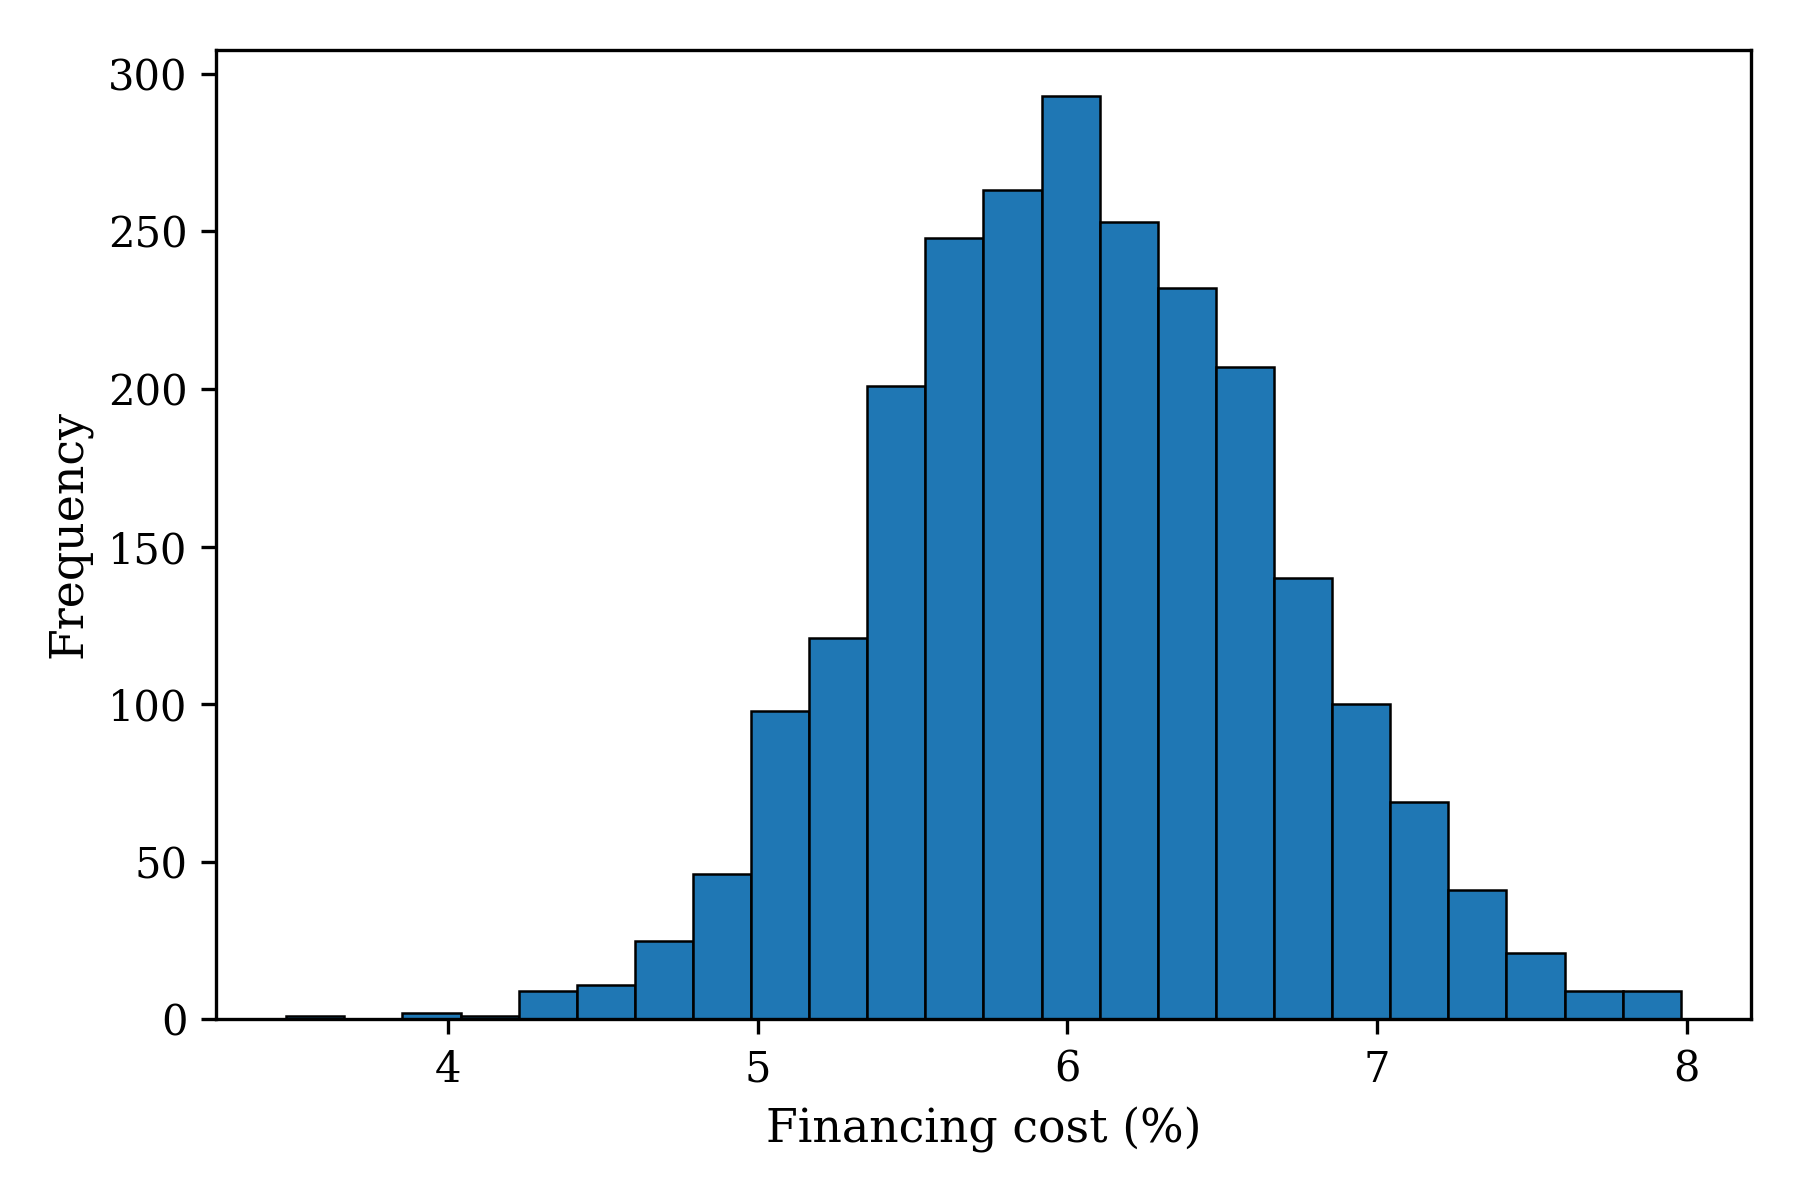
\includegraphics[width=10.16cm,height=6.77cm]{./images/fig1a.png}\\
\textbf{Panel B. Disclosure Quality}\\
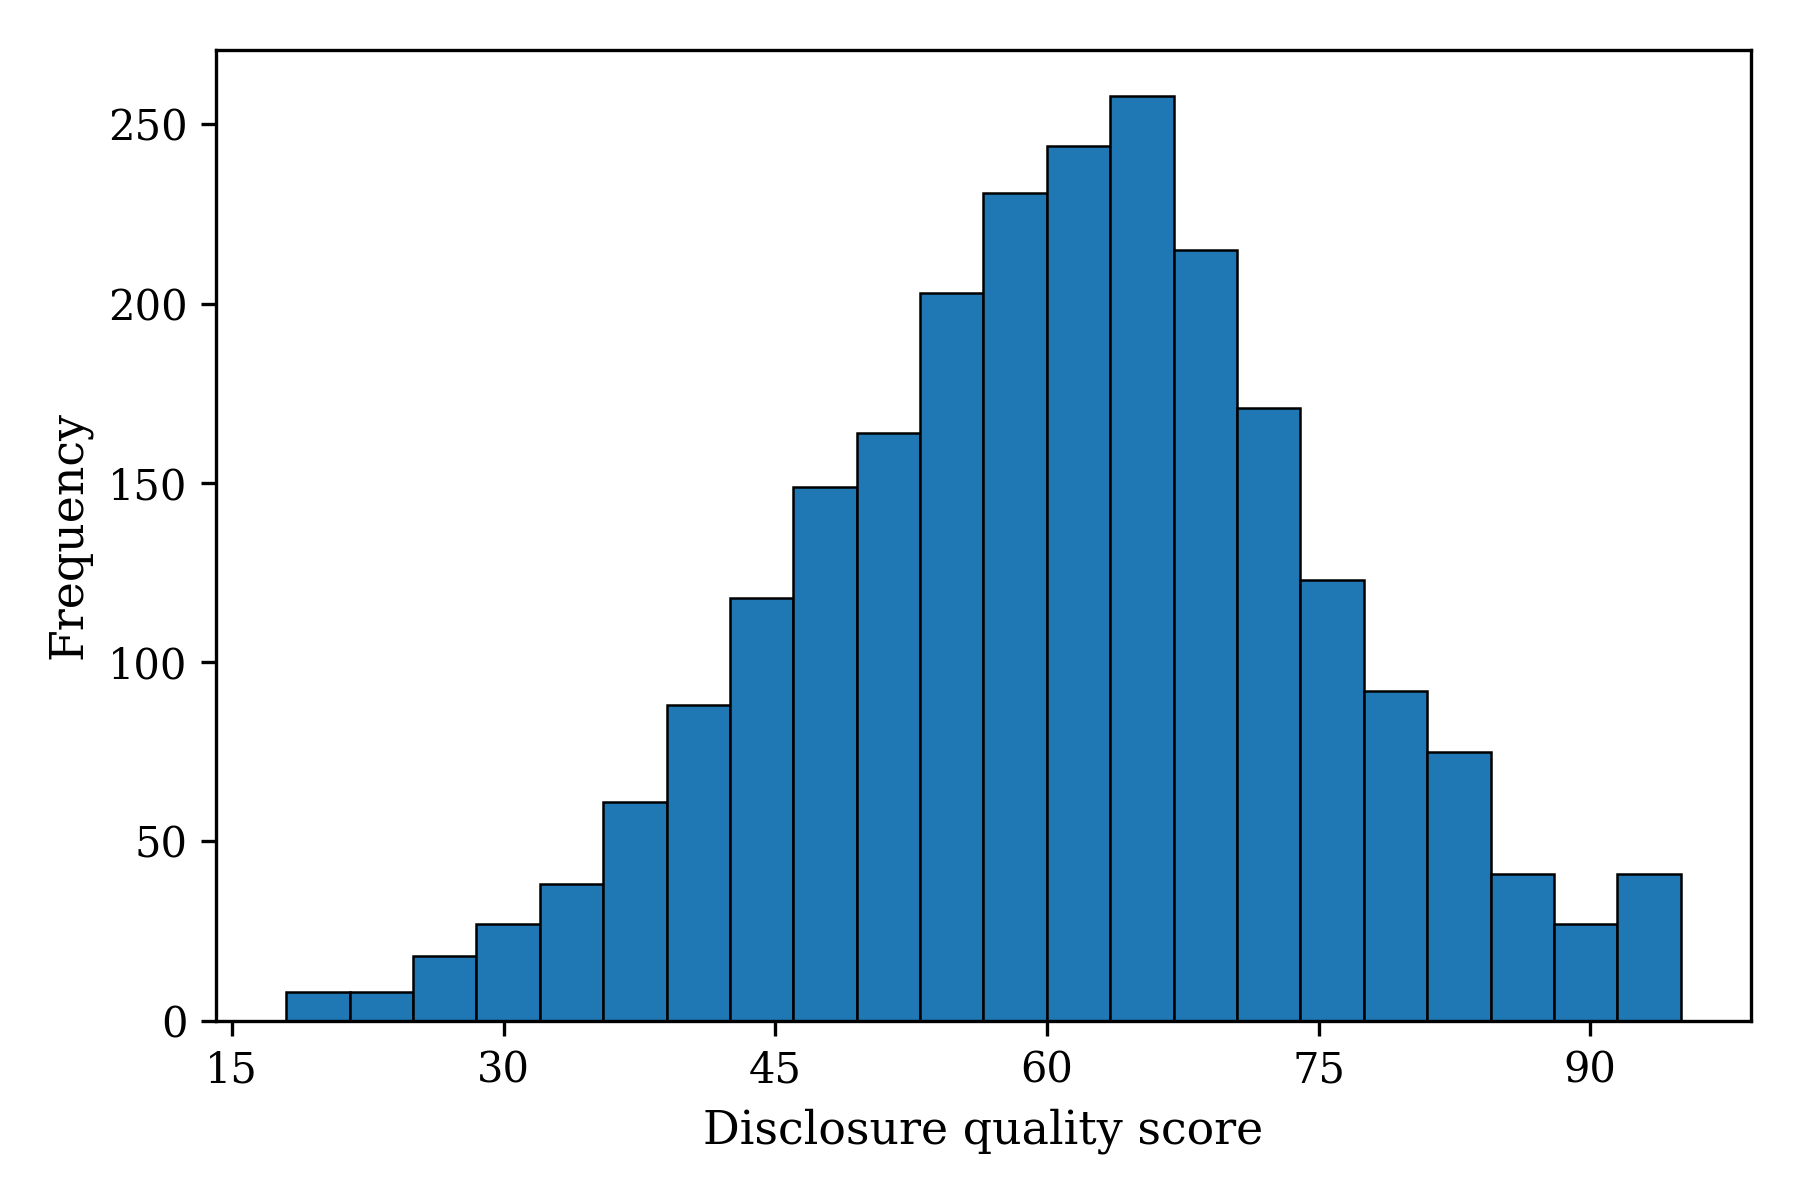
\includegraphics[width=10.16cm,height=6.77cm]{./images/fig1b.png}
\end{figure}

\clearpage
\begin{figure}[!htbp]
\caption{Binned Scatter Plot of Financing Cost and Disclosure Quality}
\label{fig:binned_scatter}\vspace{-2.5ex}
\floatnotes{This figure illustrates a common visual summary for the relation between the dependent variable and the main explanatory variable. The points show binned means and the solid line shows a fitted quadratic relation. In your own paper, specify whether fixed effects or controls have been partialled out before constructing the plot.}
\centering
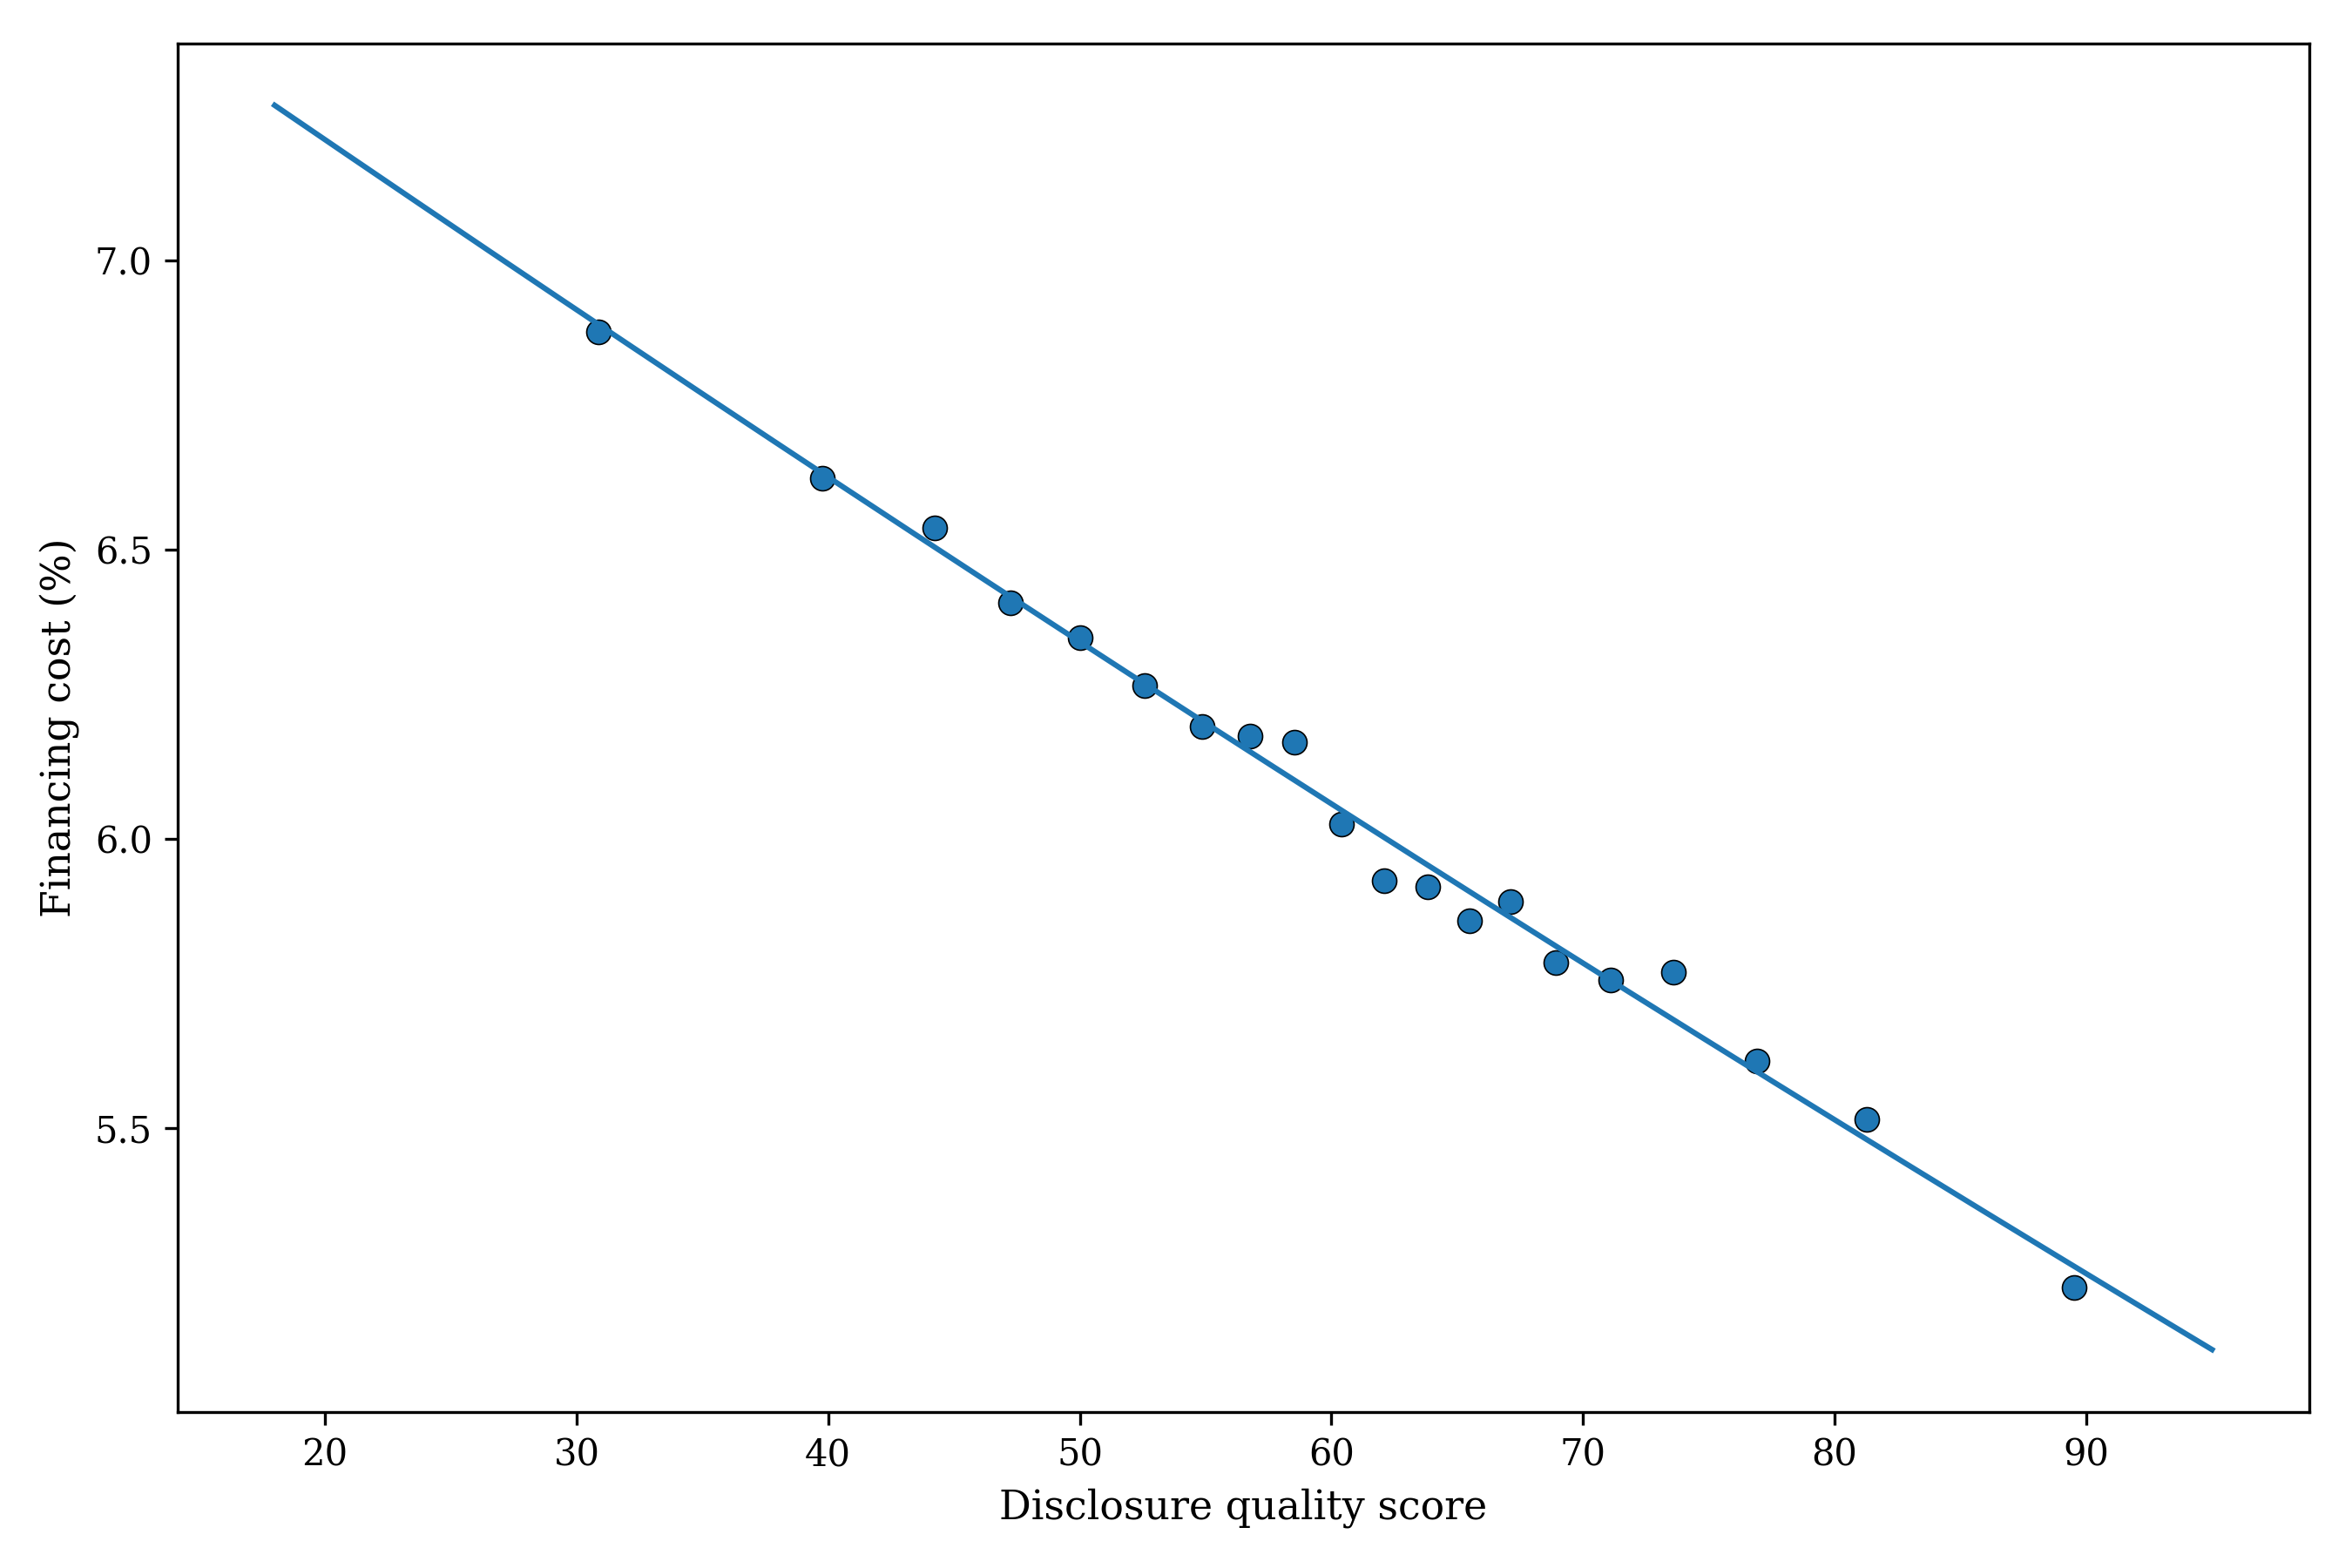
\includegraphics[width=15.24cm,height=10.16cm]{./images/fig2.png}
\end{figure}

\clearpage
\begin{figure}[!htbp]
\caption{Predicted Financing Cost by Disclosure Quality and Financial Constraint Status}
\label{fig:heterogeneity}\vspace{-2.5ex}
\floatnotes{This figure shows one way to present cross-sectional heterogeneity. The lines can be interpreted as fitted values from the interaction specification in \autoref{tab:heterogeneity}. Replace the group labels, fitted values, and confidence intervals so they match your own empirical setting.}
\centering
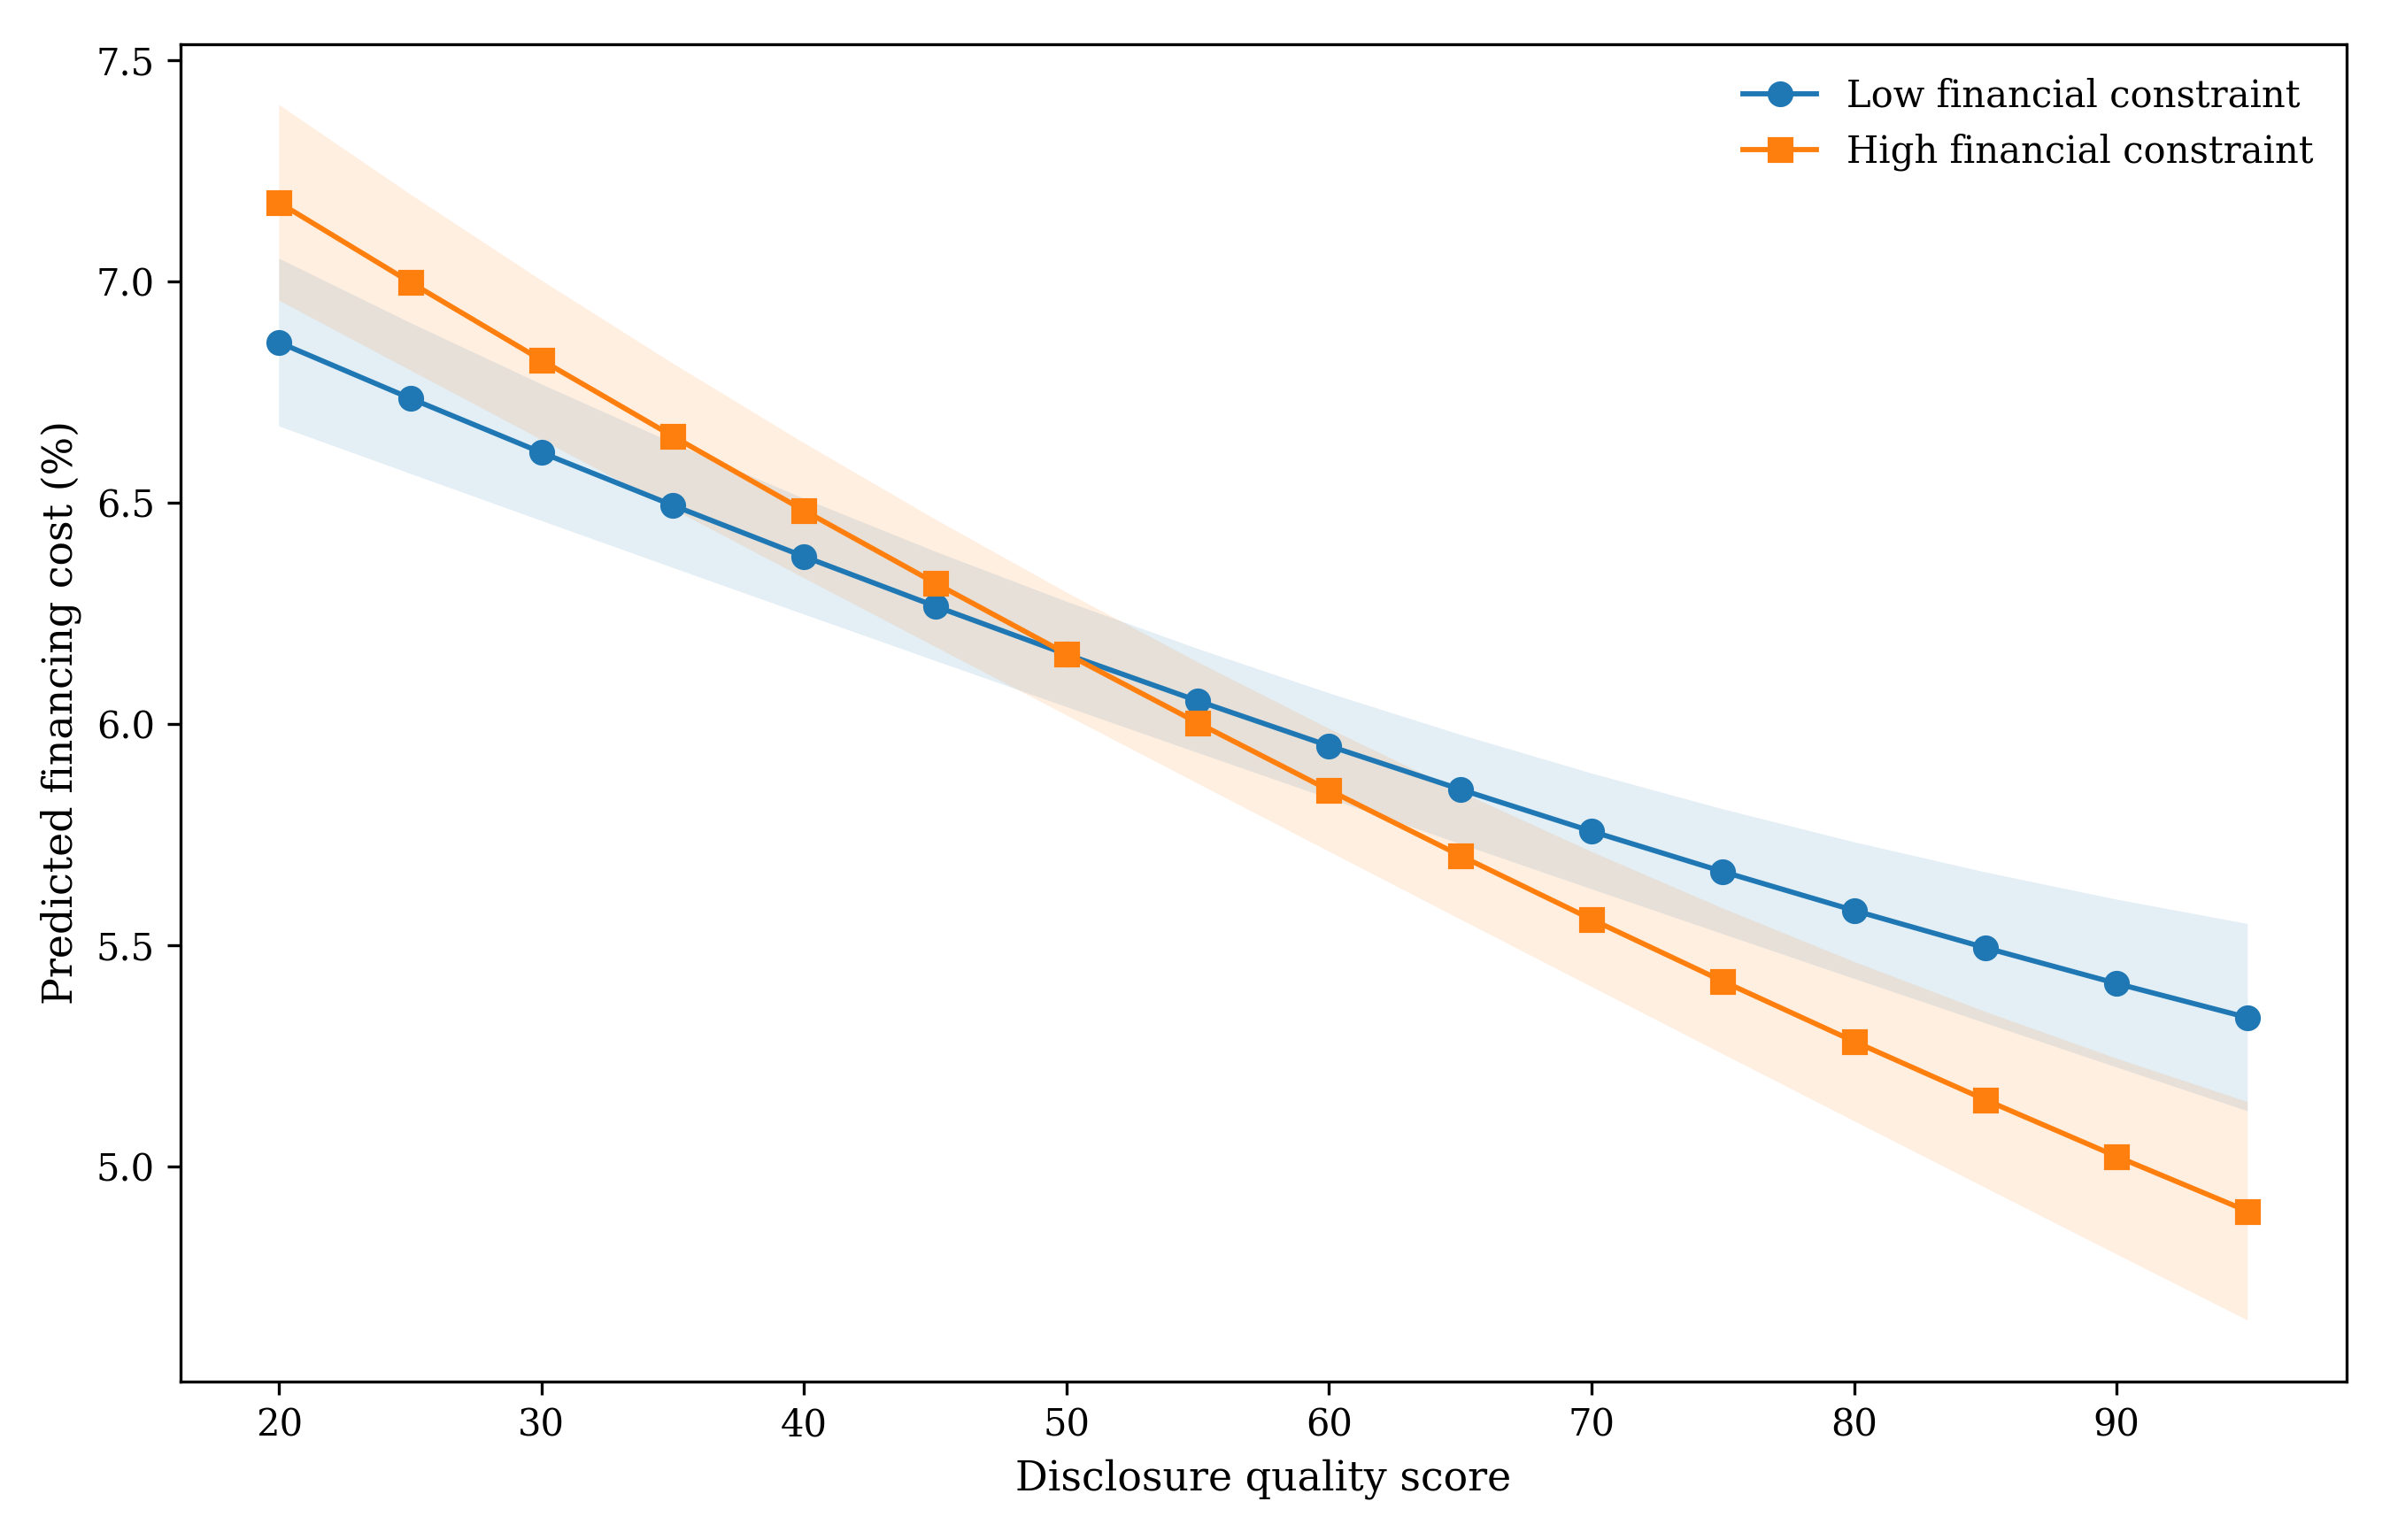
\includegraphics[width=15.24cm,height=9.6cm]{./images/fig3.png}
\end{figure}

\clearpage
\begin{figure}[!htbp]
\caption{Appendix Figure: Distribution of Regression Residuals}
\label{fig:appendix_hist}\vspace{-2.5ex}
\floatnotes{Appendix figures are useful for diagnostics, supplementary descriptive evidence, or alternative specifications. This residual histogram is included only as a formatting example.}
\centering
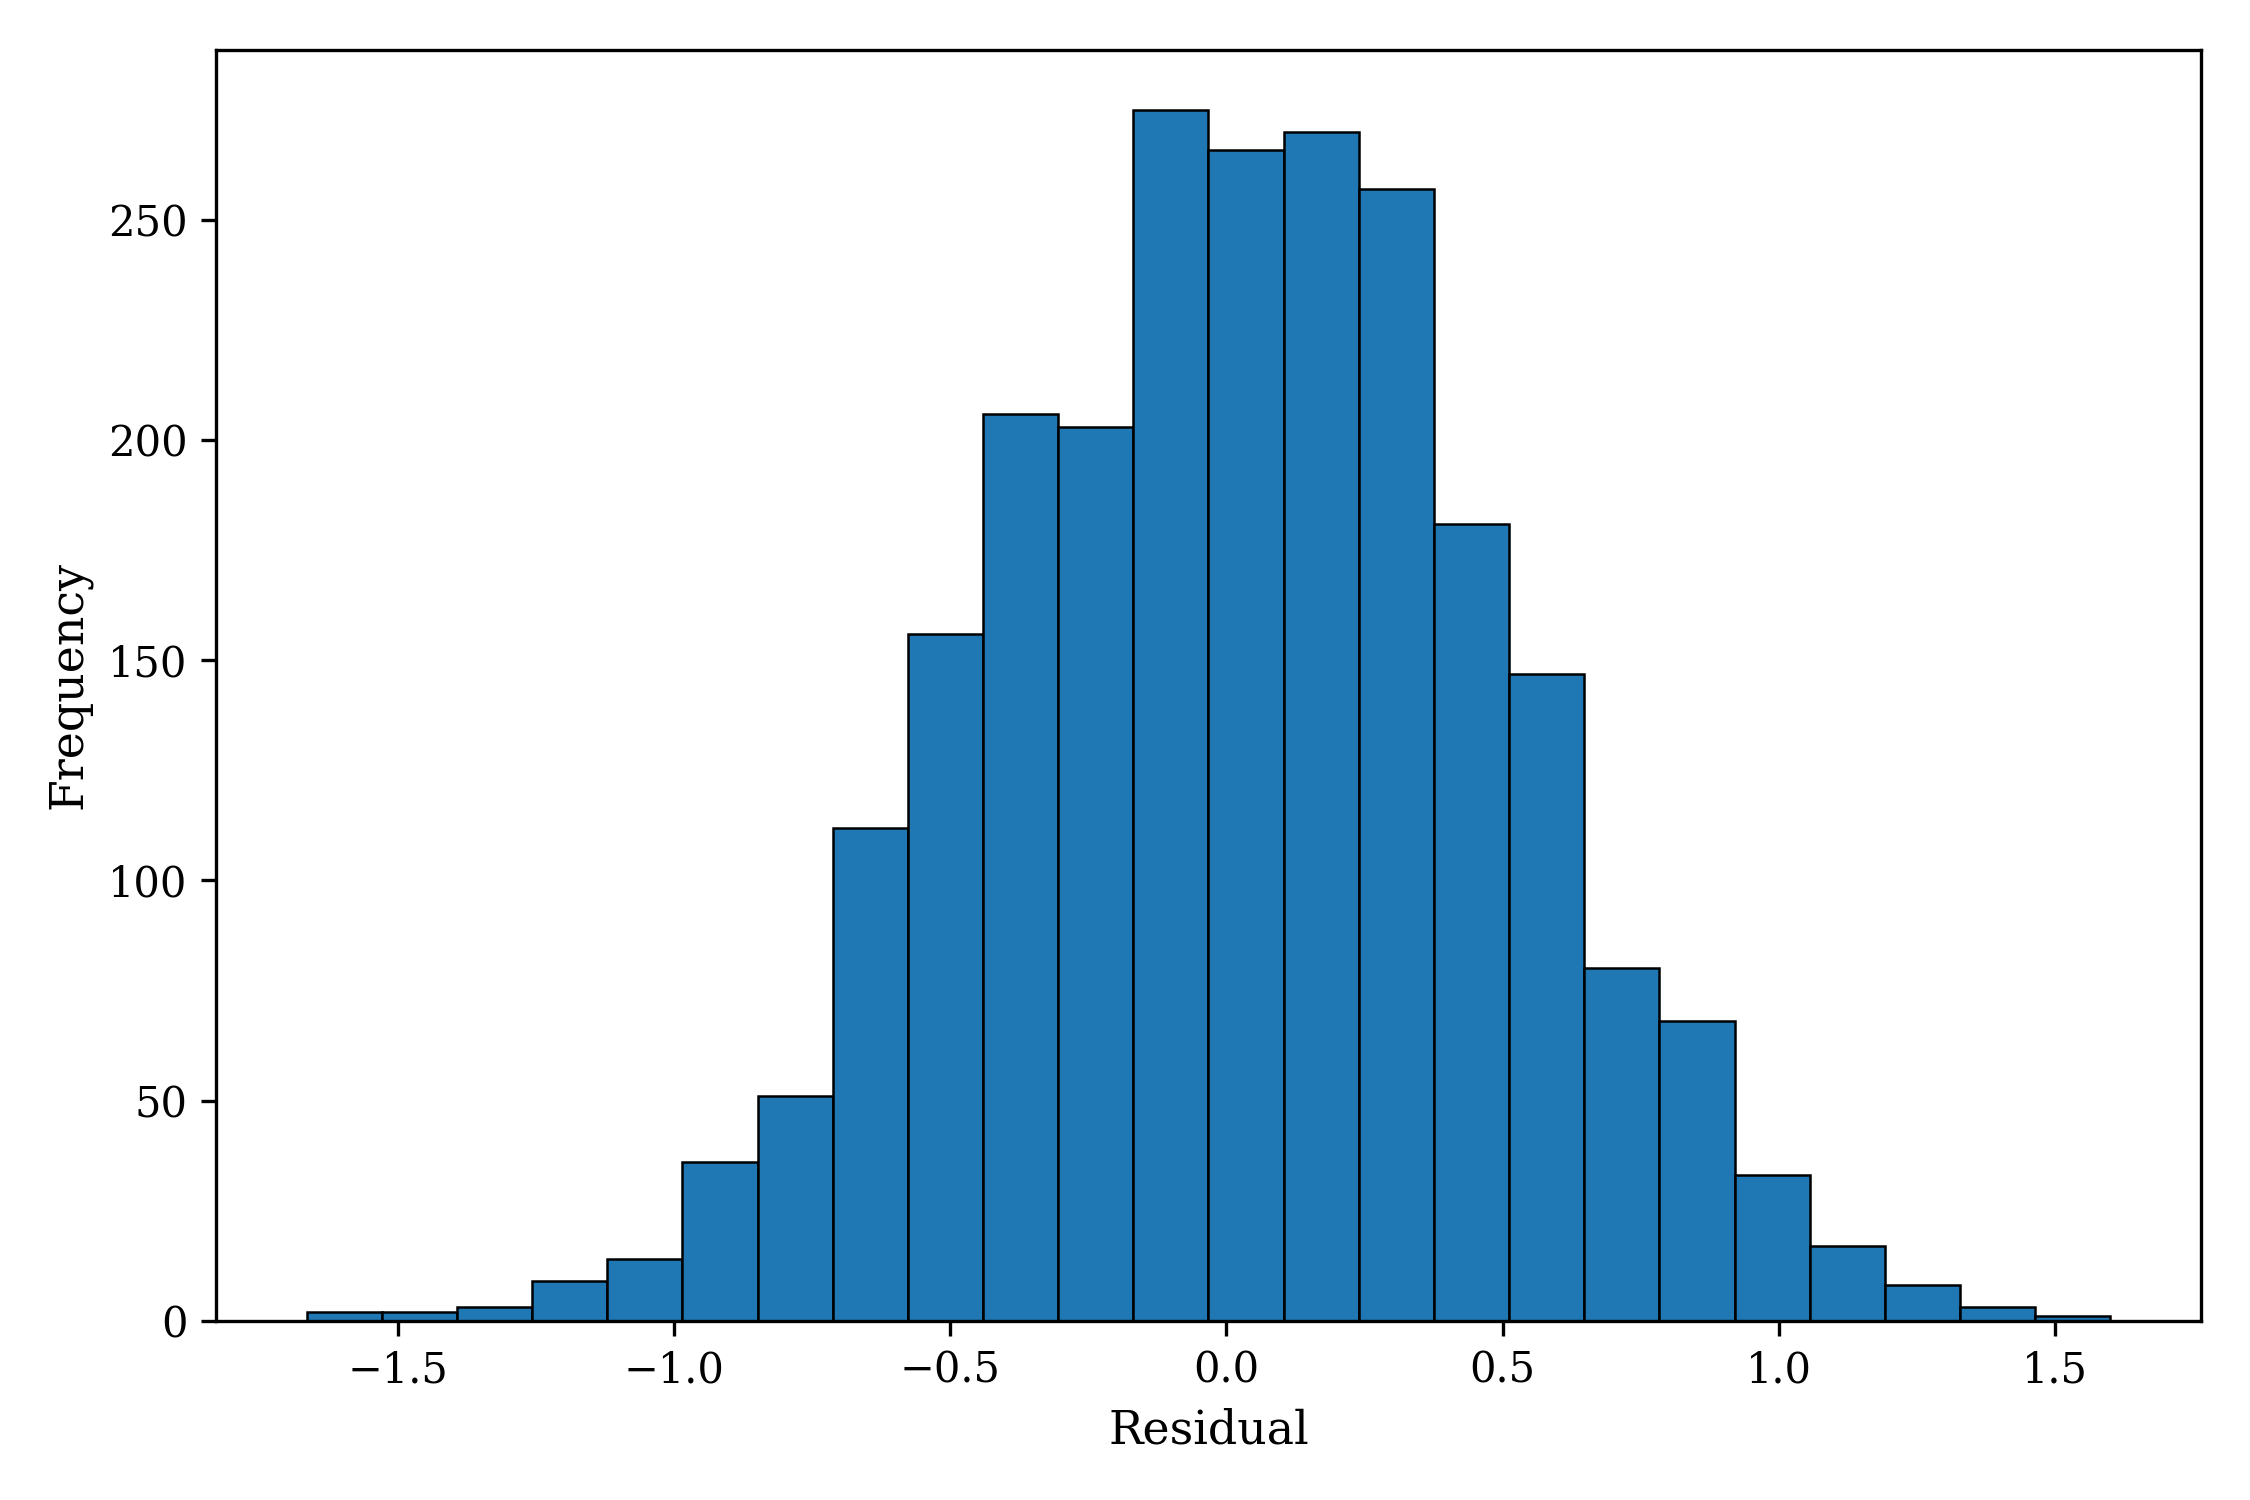
\includegraphics[width=12.8cm,height=8.5cm]{./images/figA1.png}
\end{figure}

\clearpage
\begin{table}[!htbp]
\centering
\caption{Summary Statistics}
\label{tab:summary}\vspace{-2.5ex}
\floatnotes{This table illustrates a standard summary-statistics layout with an optional second panel for correlations. Replace the variable labels, sample description, and descriptive moments with your own data. Panel A reports means, standard deviations, and selected distributional statistics. Panel B reports simple pairwise correlations among core variables.}
\setlength{\tabcolsep}{5pt}
\small

\textbf{Panel A. Descriptive Statistics}
\begin{tabularx}{\textwidth}{@{}Xrrrrrr@{}}
\\
\toprule
\textbf{Variable} & \textbf{Mean} & \textbf{SD} & \textbf{P25} & \textbf{Median} & \textbf{P75} & \textbf{N} \\
\midrule
Financing Cost (\%) & 5.87 & 1.12 & 5.08 & 5.83 & 6.61 & 2,400 \\
Disclosure Quality & 61.40 & 14.20 & 51.00 & 62.00 & 72.00 & 2,400 \\
Ln(Assets) & 7.93 & 1.12 & 7.14 & 7.88 & 8.70 & 2,400 \\
Leverage & 0.29 & 0.17 & 0.15 & 0.28 & 0.41 & 2,400 \\
Profitability & 0.11 & 0.07 & 0.06 & 0.10 & 0.15 & 2,400 \\
Market-to-Book & 1.84 & 0.76 & 1.29 & 1.73 & 2.24 & 2,400 \\
Tangibility & 0.31 & 0.16 & 0.18 & 0.30 & 0.42 & 2,400 \\
Analyst Coverage & 12.70 & 7.80 & 6.00 & 11.00 & 18.00 & 2,400 \\
\bottomrule
\\
\end{tabularx}

\medskip
\textbf{Panel B. Correlation Matrix}

\footnotesize
\begin{tabularx}{\textwidth}{@{}X*{6}{r}@{}}
\\
\toprule
 & (1) & (2) & (3) & (4) & (5) & (6) \\
\midrule
(1) Financing Cost & 1.00 &  &  &  &  &  \\
(2) Disclosure Quality & -0.31 & 1.00 &  &  &  &  \\
(3) Ln(Assets) & -0.18 & 0.21 & 1.00 &  &  &  \\
(4) Leverage & 0.27 & -0.12 & 0.09 & 1.00 &  &  \\
(5) Profitability & -0.24 & 0.16 & 0.11 & -0.21 & 1.00 &  \\
(6) Analyst Coverage & -0.14 & 0.23 & 0.33 & -0.05 & 0.10 & 1.00 \\
\bottomrule
\\
\end{tabularx}

\end{table}

\clearpage
\begin{table}[!htbp]
\centering
\caption{Disclosure Quality and Financing Cost: Baseline Regressions}
\label{tab:baseline}\vspace{-2.5ex}
\floatnotes{This table illustrates a common regression format for empirical finance papers. The dependent variable is financing cost in percentage points. All coefficients, test statistics, and goodness-of-fit measures are placeholders intended only to preserve style and layout. t-statistics appear in parentheses.}
\small
\begin{tabular}{lcccc}
\toprule
 & \multicolumn{4}{c}{Dependent Variable: Financing Cost (\%)} \\
\cmidrule(lr){2-5}
 & (1) & (2) & (3) & (4) \\
\midrule
Disclosure Quality & -0.018\sym{***} & -0.015\sym{***} & -0.013\sym{***} & -0.011\sym{***} \\
 & (-5.41) & (-4.98) & (-4.36) & (-3.92) \\
[0.5ex]
Ln(Assets) &  & -0.072\sym{***} & -0.065\sym{***} & -0.049\sym{**} \\
 &  & (-3.11) & (-2.88) & (-2.14) \\
[0.5ex]
Leverage &  & 0.684\sym{***} & 0.611\sym{***} & 0.573\sym{***} \\
 &  & (4.29) & (3.98) & (3.75) \\
[0.5ex]
Profitability &  & -0.921\sym{***} & -0.808\sym{***} & -0.742\sym{***} \\
 &  & (-4.87) & (-4.33) & (-4.01) \\
[0.5ex]
Market-to-Book &  & -0.053\sym{*} & -0.041 & -0.038 \\
 &  & (-1.88) & (-1.49) & (-1.39) \\
[0.5ex]
Tangibility &  &  & 0.214\sym{*} & 0.205\sym{*} \\
 &  &  & (1.92) & (1.85) \\
[0.5ex]
Analyst Coverage &  &  & -0.009\sym{**} & -0.008\sym{*} \\
 &  &  & (-2.01) & (-1.83) \\
[0.5ex]
Constant & 6.944\sym{***} & 7.411\sym{***} & 7.205\sym{***} & 7.622\sym{***} \\
 & (19.34) & (16.28) & (14.95) & (13.67) \\
\midrule
Firm Fixed Effects & No & No & Yes & Yes \\
Year Fixed Effects & No & Yes & Yes & Yes \\
Industry-by-Year Fixed Effects & No & No & No & Yes \\
Observations & 2,400 & 2,400 & 2,400 & 2,400 \\
Adjusted \(R^2\) & 0.096 & 0.184 & 0.361 & 0.409 \\
\bottomrule
\multicolumn{5}{l}{\footnotesize \sym{*} $p<0.10$, \sym{**} $p<0.05$, \sym{***} $p<0.01$.}
\end{tabular}
\end{table}

\clearpage
\begin{table}[!htbp]
\centering
\caption{Cross-Sectional Heterogeneity}
\label{tab:heterogeneity}\vspace{-2.5ex}
\floatnotes{This table shows one way to present interactions or subgroup analyses. Columns (1) and (2) focus on financial constraints, and Columns (3) and (4) focus on analyst coverage. The entries are illustrative placeholders only.}
\small
\begin{tabular}{lcccc}
\toprule
 & (1) & (2) & (3) & (4) \\
\midrule
Disclosure Quality & -0.010\sym{***} & -0.009\sym{***} & -0.012\sym{***} & -0.011\sym{***} \\
 & (-3.51) & (-3.22) & (-4.08) & (-3.71) \\
[0.5ex]
Disclosure Quality $\times$ High Constraint & -0.009\sym{**} & -0.010\sym{**} &  &  \\
 & (-2.43) & (-2.57) &  &  \\
[0.5ex]
High Constraint & 0.284\sym{**} & 0.261\sym{**} &  &  \\
 & (2.12) & (2.02) &  &  \\
[0.5ex]
Disclosure Quality $\times$ Low Analyst Coverage &  &  & -0.007\sym{*} & -0.008\sym{**} \\
 &  &  & (-1.91) & (-2.11) \\
[0.5ex]
Low Analyst Coverage &  &  & 0.198\sym{*} & 0.216\sym{**} \\
 &  &  & (1.82) & (2.03) \\
[0.5ex]
Controls & Yes & Yes & Yes & Yes \\
Firm Fixed Effects & Yes & Yes & Yes & Yes \\
Year Fixed Effects & Yes & Yes & Yes & Yes \\
Industry-by-Year Fixed Effects & No & Yes & No & Yes \\
Observations & 2,400 & 2,400 & 2,400 & 2,400 \\
Adjusted \(R^2\) & 0.376 & 0.413 & 0.371 & 0.408 \\
\bottomrule
\multicolumn{5}{l}{\footnotesize t-statistics in parentheses. \sym{*} $p<0.10$, \sym{**} $p<0.05$, \sym{***} $p<0.01$.}
\end{tabular}
\end{table}

\clearpage
\begin{table}[!htbp]
\centering
\caption{Appendix Table: Variable Definitions}
\label{tab:appendix_variables}\vspace{-2.5ex}
\floatnotes{Appendix tables are a convenient place for compact variable definitions, coding details, or sample-construction notes. Replace the entries below with definitions that match your project.}
\small
\begin{tabularx}{\textwidth}{@{}L{3.0cm}X@{}}
\toprule
\textbf{Variable} & \textbf{Definition} \\
\midrule
Financing Cost & Example dependent variable measured in percentage points. This can stand in for a bond spread, loan spread, cost of debt, implied cost of equity, capitalization rate, or any other outcome relevant to the paper. \\
Disclosure Quality & Example explanatory variable scaled from 0 to 100. Replace with your focal treatment, exposure, shock, or continuous explanatory measure. \\
Ln(Assets) & Natural logarithm of total assets or an analogous size proxy. \\
Leverage & Ratio of total debt to total assets. \\
Profitability & Return on assets or another operating-performance measure. \\
Market-to-Book & Placeholder proxy for growth opportunities or valuation. \\
Tangibility & Ratio of tangible assets to total assets. \\
Analyst Coverage & Number of analysts following the firm. \\
High Constraint & Indicator equal to one for observations classified as financially constrained under your preferred proxy. \\
\bottomrule
\end{tabularx}
\end{table}

\end{document}
